\documentclass{math}

\usepackage{graphicx}

\title{Introduction to Cryptography}
\author{Alvin Lin}
\date{January 2018 - May 2018}

\begin{document}

\maketitle

\section*{Ciphers and Cryptosystems}

\subsection*{Hill Cipher}
The Hill Cipher was developed by Lester Hill in 1929. It's strength was that it
completely hid single-letter frequencies. It was strong against a
ciphertext-only attack but easily broken by a known plaintext attack. The Hill
cipher is done by taking a matrix as the key:
\[ K = \begin{bmatrix}2 & 1 \\ 1 & 1\end{bmatrix} \]
Given the plaintext HELP, we split it into \( 1\times2 \) column vectors so
that they can be multiplied by the key vector:
\[ \begin{bmatrix}H \\ E\end{bmatrix},
  \begin{bmatrix}L \\ P\end{bmatrix}\to
  \begin{bmatrix}7 \\ 4\end{bmatrix},
  \begin{bmatrix}11 \\ 15\end{bmatrix} \]
The ciphertext is produced by multiplying the key matrix with the column
vectors.
\begin{align*}
  \begin{bmatrix}2 & 1 \\ 1 & 1\end{bmatrix}
    \begin{bmatrix}7 \\ 4\end{bmatrix} &\equiv
    \begin{bmatrix}18 \\ 11\end{bmatrix}\mod(26) \\
  \begin{bmatrix}2 & 1 \\ 1 & 1\end{bmatrix}
    \begin{bmatrix}11 \\ 15\end{bmatrix} &\equiv
    \begin{bmatrix}11 \\ 0\end{bmatrix}\mod(26)
\end{align*}
This yields the cipher text 18-11-11-0 or RKKA. Decryption is done by computing
the inverse of the key matrix \( K^{-1} \) and repeating the same process.

\subsection*{Stream Ciphers}
Stream ciphers were invented in 1917 by Gilbert Vernam. It involves a plaintext
\( x \) and a key stream \( k \) to yield a ciphertext \( y \). Encryption
and decryption operations are simple additions modulo 2 (aka XOR).
\begin{itemize}
  \item Encryption: \( y_i = x_i+k_i\mod2 \)
  \item Decryption: \( x_i = y_i+k_i\mod2 \)
\end{itemize}
Stream ciphers encrypt bits individually. They're usually small and fast, and
are common in embedded devices. Block ciphers on the other hand, encrypt whole
blocks of information and are common for Internet applications. The security of
stream ciphers depend entirely on the key stream. The key stream \( k \) should
be random, but reproducible by the sender and the receiver. \textbf{Synchronous}
stream ciphers use a key stream that only depends on the key, while
\textbf{asynchronous} stream ciphers use a key stream that also depends on the
ciphertext.

\subsection*{Random Number Generators}
Random number generators are needed in cryptography, particularly for stream
ciphers. There are three types: true random number generators, pseudorandom
number generators, and cryptographically secure random number generators. The
basic requirements for randomness:
\begin{itemize}
  \item Uniform Distribution (The frequency of occurrence of ones and zeroes
  should be approximately equal)
  \item Independence (Each bit should be uncorrelated with all previous bits)
\end{itemize}
For cryptography, the compromise of one output must not compromise future or
previous outputs.

\subsubsection*{True Random Number Generators}
True random number generators are based on some random physical processes, such
as coin flipping, dice rolling, semiconductor noise, radioactive decay, mouse
movement, or clock jitter of digital circuits. The output stream should have
good statistical properties and should not be able to be predicted or
reproduced. These are typically used for the generation of keys and nonces.

\subsubsection*{Pseudorandom Number Generators}
Pseudorandom number generators are algorithms used to produce an open-ended
sequence of bits. They generate sequences from an initial seed value. The output
stream has good statistical properties and can typically be reproduced and
predicted.
\par The basic requirement when a pseudorandom number generator or pseudorandom
function is used for a cryptographic application is that an adversary who does
not know the seed is unable to determine the pseudorandom string. The bit stream
should appear random even though it is deterministic, and should have no
correlation with the seed.

\subsubsection*{Linear Congruential Generator}
The linear congruential generator is an algorithm first proposed by Lehmer
parameterized with four numbers \( a,b,m,seed \). The sequence of random
numbers \( x_n \) is obtained via the following iterative equation:
\[ x_{n+1} = (ax_n+b)\mod(m) \]
This has bad cryptographic properties due to its linearity.

\subsection*{One-Time Pad}
The one-time pad was an improvement to the Vernam cipher propsed by Army
Signal Corp officer Joseph Mauborgne. It uses and random key that is as long
as the message so that the key does not need to be repeated. The key is used
to encrypt and decrypt a single message and then is discarded. Each new message
requires a new key of the same length as the new message.
\par This scheme is unbreakable because it produces random output with no
statistical relationship to the plaintext. The one-time pad offers complete
security but has fundamental problems, namely key distribution and key
generation. Thus, the one-time pad is useful primarily only in low-bandwidth
channels requiring very high security.

\subsection*{Linear Feedback Shift Registers (LSFR)}
Linear feedback shift registers are cascades of flip flops, sharing the same
clock, whose input bit is a linear function of its previous state. The feedback
portion computes fresh input bits by calculating the XOR of certain state bits.
Their degree is given by the number of storage elements \( m \), with the
maximum output length being \( 2^m-1 \). Linear feedback shift registers are
typically described by polynomials:
\[ P(x) = x^m+p_{m-1}x^{m-1}+\dots+p_2x^2+p_1x+x_0 \]
Single linear feedback shift registers generate highly predictable output. If
\( 2m \) output bits of a linear shift feedback register of degree \( m \) are
known, the feedback coefficients \( p_i \) can be found by solving a system of
linear equations. Because of this, most stream ciphers use combinations of
stream ciphers.

\subsection*{RC4 Stream Cipher}
The RC4 stream cipher was designed by Ron Rivest for RSA Data Security in 1987.
The algorithm had been a trade secret, allegedly revealed on the Internet in
1994. The design of RC4 avoids the use of LSFRs and is ideal for software
implementation. RC4 generates a keystream (pseudorandom stream of bits), that is
used for encryption by combining it with the plaintext using the XOR gate
(similar to the Vernam cipher).
\begin{itemize}
  \item Input: key (typically from 40 to 2048 bits)
  \item Heart: S-box - a permutation of all 256 possible bytes
  \item Output: a pseudo-random keystream in bytes
\end{itemize}
The RC4 cipher has two components, a key scheduling algorithm (KSA) and a
pseudo-random generation algorithm (PRGA).

\subsection*{Block Ciphers}
A stream cipher algorithm defines how to encrypt or decrypt arbitrary length
messages. A block cipher can only encrypt or decrypt \( b \) bits, no more, no
less. Arbitrary length message are handled by a separate algorithm called a
block cipher mode of operation (ECB). A stream cipher's encryption and
decryption operations are the same. A block cipher's encryption and decryption
operations are different. To decrypt, the encryption operation must be run
backward. Thus, the encryption operation must be invertible. Additionally, block
ciphers are much more than just an encryption algorithm, they can be used:
\begin{itemize}
  \item to build different types of block-based encryption schemes
  \item to realize stream ciphers
  \item to construct hash functions
  \item to make message authentication codes
  \item to build key establishment protocols
  \item to make a pseudo-random number generator
\end{itemize}

\subsubsection*{Block Cipher Primitives}
Claude Shannon: there are two primitive operations with which strong encryption
algorithms can be built.
\begin{enumerate}
  \item \textbf{Confusion:} An encryption operation where the relationship
  between the key and ciphertext is obscured. Today, a common element for
  achieving confusion is substitution, which is found in both AES and DES.
  \item \textbf{Diffusion:} An encryption operation where the influence of one
  plaintext symbol is spread of over many ciphertext symbols with the goal of
  hiding statistical properties of the plaintext. A simple diffusion element is
  the bit permutation, which is frequently used within DES. This obscures the
  relationship between the ciphertext and the plaintext.
\end{enumerate}
Both operations by themselves cannot provide security. The idea is to
concatenate confusion and diffusion elements to build so called product ciphers.
Most of today's block ciphers are product ciphers as they consist of rounds
which are applied repeatedly to the data. This can reach excellent diffusion, as
changing one bit of the plaintext results on average in the change of half the
output bits.

\subsection*{Block Cipher Modes of Operation}
There are several ways of encrypting long plaintexts with a block cipher:
\begin{itemize}
  \item Electronic Code Book mode (ECB)
  \item Cipher Block Chaining mode (CBC)
  \item Output Feedback mode (OFB)
  \item Cipher Feedback mode (CFB)
  \item Counter mode (CTR)
  \item Galois Counter Mode (GCM)
\end{itemize}
These modes have the goal of providing authenticity and integrity in addition to
confidentiality. It ascertains that the message is coming from the original
sender and that it was not altered during transmission.

\subsubsection*{Electronic Code Book mode (ECB)}
This is the simplest of the encryption modes. Messages which exceed \textit{b}
bits are partitioned into \textit{b}-bit blocks, which are encrypted separately.
In case the plaintext message's length is not a multiple of \textit{b}, we add
padding to the end.
\begin{center}
  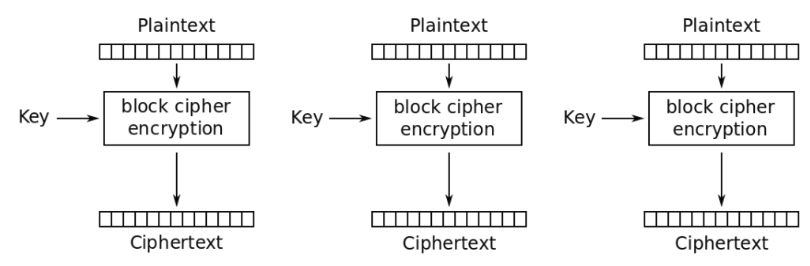
\includegraphics[width=12cm]{assets/ecb.png}
\end{center}
\textbf{Advantages:}
\begin{itemize}
  \item No block synchronization between the sender and receiver is required.
  \item Bit errors caused by noisy channels only affect the corresponding block
  but not succeeding blocks.
  \item Encryption can be parallelized, which is an advantage for high-speed
  implementations.
\end{itemize}
\textbf{Disadvantages:}
\begin{itemize}
  \item Encryption is highly deterministic.
  \item Identical plaintexts result in identical ciphertexts.
  \item An attacker recognizes if the same message has been sent twice.
  \item Plaintext blocks are encrypted independently of previous blocks.
  \item An attacker may reorder ciphertext blocks which result in valid
  plaintext.
  \item Statistical properties in the plaintext are preserved in the
  ciphertext.
\end{itemize}
Once a particular plaintext to ciphertext block mapping is known, a sequence of
ciphertext blocks can easily be manipulated.

\subsubsection*{Cipher Block Chaining mode (CBC)}
There are two main ideas behind this mode: the encryption of all blocks are
chained together, and the encryption is randomized by using an initialization
vector.
\begin{center}
  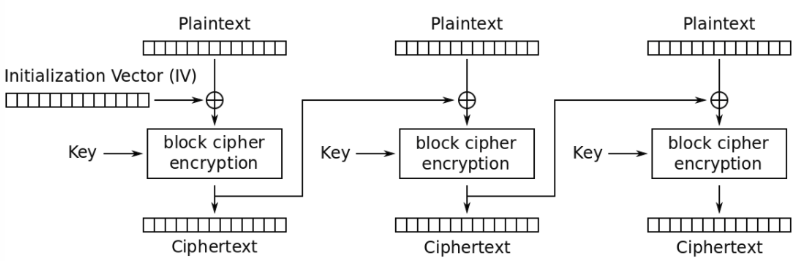
\includegraphics[width=12cm]{assets/cbc.png}
\end{center}
This mode also requires padding, but messages longer than \( 2^{\frac{n}{2}} \)
blocks (where \( n \) is the block size in bits) shouldn't be encrypted with
this mode, since it gives an attacker more information about the ciphertext.
Encryption cannot be parallelized, but decryption can be. The initialization
vector does not need to be secret, but it should be a randomized nonce.

\subsubsection*{Output Feedback mode (OFB)}
This mode builds a synchronous stream cipher from a block cipher, where the key
stream is generated in a blockwise fashion. The output of the cipher gives us
key stream bits with which we can encrypt plaintext bits using the XOR
operation. This mode also requires an initialization vector (which also should
be a randomized nonce).
\begin{center}
  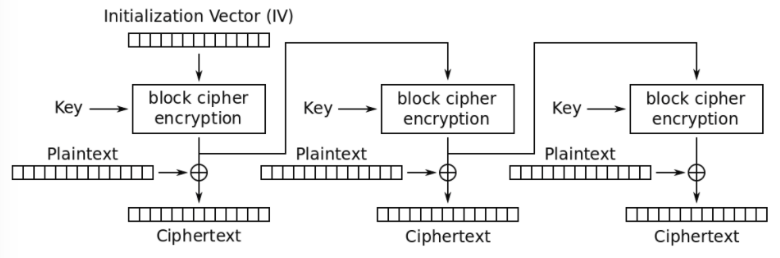
\includegraphics[width=12cm]{assets/ofb.png}
\end{center}

\subsubsection*{Cipher Feedback mode (CFB)}
This mode uses a block cipher as a building block for an synchronous stream
cipher. The key stream is generated in a blockwise fashion and is also a
function of the ciphertext. Since it also uses a randomized initialization
vector, the ciphertext is also nondeterministic. It can be used in situations
where short plaintext blocks are to be encrypted, but has no real advantage
over Output Feedback mode.
\begin{center}
  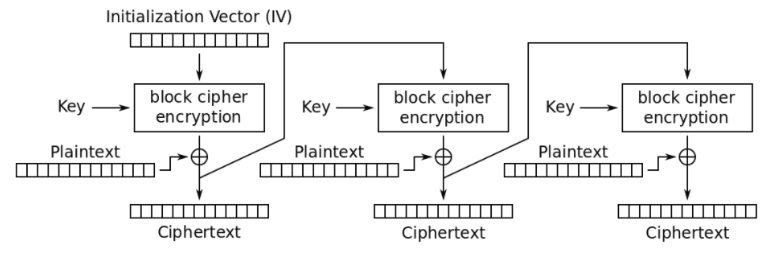
\includegraphics[width=12cm]{assets/cfb.png}
\end{center}

\subsubsection*{Counter mode (CTR)}
This mode turns a block cipher into a stream cipher where the keystream is
computed in a blockwise fashion (similar to OFB and CFB mode). The input to the
block cipher is a counter which assumes a different value every time the block
cipher computes a new key stream block. Unlike CFB, and OFB however, this is
highly parallelizable and does not require padding since the unneeded portion
of the last key block can be discarded (because it is a stream cipher).
\begin{center}
  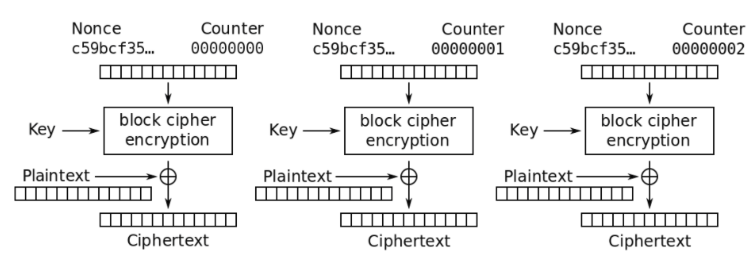
\includegraphics[width=12cm]{assets/ctr.png}
\end{center}

\subsection*{Feistel Cipher (Feistel network)}
Horst Feistel proposed the use of a cipher that alternates substitutions and
permutations. This is a practical application of a proposal by Claude Shannon to
develop a product cipher. A large set of block ciphers use the scheme (it is a
design model from which many different block ciphers are derived), including the
Data Encryption Standard (DES). DES is just one example of a Feistel Cipher.

\subsection*{DES Algorithm}
DES Facts:
\begin{itemize}
  \item Data Encryption Standard (DES) encrypts blocks of size 64 bit.
  \item Developed by IBM based on the cipher Lucifer under the influence of the
  National Security Agency (NSA).
  \item Standardized in 1977 by the National Bureau of Standards (NBS), now
  called the National Institute of Standards and Technology (NIST).
  \item Most popular block cipher for most of the last 30 years.
  \item By far the best studied symmetric algorithm.
  \item Nowadays considered insecure due to the small key length of 56 bits.
  \item Replaced by the Advanced Encryption Standard (AES) in 2000.
\end{itemize}
The DES algorithm encrypts 64-bit blocks using a 56-bit key. It is a symmetric
cipher, so it uses the same key for encryption and decryption. It uses 16 rounds
which all perform the same operation. A different subkey derived from the main
key is used in each round. DES is quite robust against known analytical attacks.
In practice, it is very difficult to break the cipher with linear or analytical
cryptanalysis. By encrypting with DES three times in a row, triple DES (3DES)
was created, against which no practical attack is currently known. 3DES is still
widely in use today.

\subsubsection*{Exhaustive Key Search}
A simple exhaustive search for a DES key pair knowing one plaintext-ciphertext
pair requires has a key space of size \( 2^56 \). However, for most other block
ciphers, a key search is somewhat more complicated. A brute-force attack can
produce false positive results, where a key is found that is not the one used
for the encryption. The likelihood of this is related to the relative size of
the key space and the plaintext space.

\subsubsection*{Example}
Assume a cipher with a block width of 64 bits and a key size of 80 bits is used
to encrypt a plaintext. If we encrypt once under all possible \( 2^80 \) keys,
we obtain \( 2^80 \) possible ciphertexts. However, there exist only \( 2^64 \)
different ones. If we run through all keys for a given plaintext-ciphertext
pairs, we find on average \( \frac{2^80}{2^64} = 2^16 \) keys that perform the
mapping \( e_k(x) = y \). Given a block cipher with a key length of \( k \)
bits and a block size of \( n \) bits, as well as \( t \) plaintext-ciphertext
pairs, the expected number of false keys which encrypts all plaintexts to the
corresponding ciphertexts is:
\[ 2^{k-tn} \]


\begin{center}
  You can find all my notes at \url{http://omgimanerd.tech/notes}. If you have
  any questions, comments, or concerns, please contact me at
  alvin@omgimanerd.tech
\end{center}

\end{document}
